% Options for packages loaded elsewhere
\PassOptionsToPackage{unicode}{hyperref}
\PassOptionsToPackage{hyphens}{url}
\PassOptionsToPackage{dvipsnames,svgnames,x11names}{xcolor}
%
\documentclass[
  letterpaper,
  DIV=11,
  numbers=noendperiod]{scrreprt}

\usepackage{amsmath,amssymb}
\usepackage{iftex}
\ifPDFTeX
  \usepackage[T1]{fontenc}
  \usepackage[utf8]{inputenc}
  \usepackage{textcomp} % provide euro and other symbols
\else % if luatex or xetex
  \usepackage{unicode-math}
  \defaultfontfeatures{Scale=MatchLowercase}
  \defaultfontfeatures[\rmfamily]{Ligatures=TeX,Scale=1}
\fi
\usepackage{lmodern}
\ifPDFTeX\else  
    % xetex/luatex font selection
\fi
% Use upquote if available, for straight quotes in verbatim environments
\IfFileExists{upquote.sty}{\usepackage{upquote}}{}
\IfFileExists{microtype.sty}{% use microtype if available
  \usepackage[]{microtype}
  \UseMicrotypeSet[protrusion]{basicmath} % disable protrusion for tt fonts
}{}
\makeatletter
\@ifundefined{KOMAClassName}{% if non-KOMA class
  \IfFileExists{parskip.sty}{%
    \usepackage{parskip}
  }{% else
    \setlength{\parindent}{0pt}
    \setlength{\parskip}{6pt plus 2pt minus 1pt}}
}{% if KOMA class
  \KOMAoptions{parskip=half}}
\makeatother
\usepackage{xcolor}
\setlength{\emergencystretch}{3em} % prevent overfull lines
\setcounter{secnumdepth}{5}
% Make \paragraph and \subparagraph free-standing
\ifx\paragraph\undefined\else
  \let\oldparagraph\paragraph
  \renewcommand{\paragraph}[1]{\oldparagraph{#1}\mbox{}}
\fi
\ifx\subparagraph\undefined\else
  \let\oldsubparagraph\subparagraph
  \renewcommand{\subparagraph}[1]{\oldsubparagraph{#1}\mbox{}}
\fi

\usepackage{color}
\usepackage{fancyvrb}
\newcommand{\VerbBar}{|}
\newcommand{\VERB}{\Verb[commandchars=\\\{\}]}
\DefineVerbatimEnvironment{Highlighting}{Verbatim}{commandchars=\\\{\}}
% Add ',fontsize=\small' for more characters per line
\usepackage{framed}
\definecolor{shadecolor}{RGB}{241,243,245}
\newenvironment{Shaded}{\begin{snugshade}}{\end{snugshade}}
\newcommand{\AlertTok}[1]{\textcolor[rgb]{0.68,0.00,0.00}{#1}}
\newcommand{\AnnotationTok}[1]{\textcolor[rgb]{0.37,0.37,0.37}{#1}}
\newcommand{\AttributeTok}[1]{\textcolor[rgb]{0.40,0.45,0.13}{#1}}
\newcommand{\BaseNTok}[1]{\textcolor[rgb]{0.68,0.00,0.00}{#1}}
\newcommand{\BuiltInTok}[1]{\textcolor[rgb]{0.00,0.23,0.31}{#1}}
\newcommand{\CharTok}[1]{\textcolor[rgb]{0.13,0.47,0.30}{#1}}
\newcommand{\CommentTok}[1]{\textcolor[rgb]{0.37,0.37,0.37}{#1}}
\newcommand{\CommentVarTok}[1]{\textcolor[rgb]{0.37,0.37,0.37}{\textit{#1}}}
\newcommand{\ConstantTok}[1]{\textcolor[rgb]{0.56,0.35,0.01}{#1}}
\newcommand{\ControlFlowTok}[1]{\textcolor[rgb]{0.00,0.23,0.31}{#1}}
\newcommand{\DataTypeTok}[1]{\textcolor[rgb]{0.68,0.00,0.00}{#1}}
\newcommand{\DecValTok}[1]{\textcolor[rgb]{0.68,0.00,0.00}{#1}}
\newcommand{\DocumentationTok}[1]{\textcolor[rgb]{0.37,0.37,0.37}{\textit{#1}}}
\newcommand{\ErrorTok}[1]{\textcolor[rgb]{0.68,0.00,0.00}{#1}}
\newcommand{\ExtensionTok}[1]{\textcolor[rgb]{0.00,0.23,0.31}{#1}}
\newcommand{\FloatTok}[1]{\textcolor[rgb]{0.68,0.00,0.00}{#1}}
\newcommand{\FunctionTok}[1]{\textcolor[rgb]{0.28,0.35,0.67}{#1}}
\newcommand{\ImportTok}[1]{\textcolor[rgb]{0.00,0.46,0.62}{#1}}
\newcommand{\InformationTok}[1]{\textcolor[rgb]{0.37,0.37,0.37}{#1}}
\newcommand{\KeywordTok}[1]{\textcolor[rgb]{0.00,0.23,0.31}{#1}}
\newcommand{\NormalTok}[1]{\textcolor[rgb]{0.00,0.23,0.31}{#1}}
\newcommand{\OperatorTok}[1]{\textcolor[rgb]{0.37,0.37,0.37}{#1}}
\newcommand{\OtherTok}[1]{\textcolor[rgb]{0.00,0.23,0.31}{#1}}
\newcommand{\PreprocessorTok}[1]{\textcolor[rgb]{0.68,0.00,0.00}{#1}}
\newcommand{\RegionMarkerTok}[1]{\textcolor[rgb]{0.00,0.23,0.31}{#1}}
\newcommand{\SpecialCharTok}[1]{\textcolor[rgb]{0.37,0.37,0.37}{#1}}
\newcommand{\SpecialStringTok}[1]{\textcolor[rgb]{0.13,0.47,0.30}{#1}}
\newcommand{\StringTok}[1]{\textcolor[rgb]{0.13,0.47,0.30}{#1}}
\newcommand{\VariableTok}[1]{\textcolor[rgb]{0.07,0.07,0.07}{#1}}
\newcommand{\VerbatimStringTok}[1]{\textcolor[rgb]{0.13,0.47,0.30}{#1}}
\newcommand{\WarningTok}[1]{\textcolor[rgb]{0.37,0.37,0.37}{\textit{#1}}}

\providecommand{\tightlist}{%
  \setlength{\itemsep}{0pt}\setlength{\parskip}{0pt}}\usepackage{longtable,booktabs,array}
\usepackage{calc} % for calculating minipage widths
% Correct order of tables after \paragraph or \subparagraph
\usepackage{etoolbox}
\makeatletter
\patchcmd\longtable{\par}{\if@noskipsec\mbox{}\fi\par}{}{}
\makeatother
% Allow footnotes in longtable head/foot
\IfFileExists{footnotehyper.sty}{\usepackage{footnotehyper}}{\usepackage{footnote}}
\makesavenoteenv{longtable}
\usepackage{graphicx}
\makeatletter
\def\maxwidth{\ifdim\Gin@nat@width>\linewidth\linewidth\else\Gin@nat@width\fi}
\def\maxheight{\ifdim\Gin@nat@height>\textheight\textheight\else\Gin@nat@height\fi}
\makeatother
% Scale images if necessary, so that they will not overflow the page
% margins by default, and it is still possible to overwrite the defaults
% using explicit options in \includegraphics[width, height, ...]{}
\setkeys{Gin}{width=\maxwidth,height=\maxheight,keepaspectratio}
% Set default figure placement to htbp
\makeatletter
\def\fps@figure{htbp}
\makeatother

\KOMAoption{captions}{tableheading}
\makeatletter
\@ifpackageloaded{tcolorbox}{}{\usepackage[skins,breakable]{tcolorbox}}
\@ifpackageloaded{fontawesome5}{}{\usepackage{fontawesome5}}
\definecolor{quarto-callout-color}{HTML}{909090}
\definecolor{quarto-callout-note-color}{HTML}{0758E5}
\definecolor{quarto-callout-important-color}{HTML}{CC1914}
\definecolor{quarto-callout-warning-color}{HTML}{EB9113}
\definecolor{quarto-callout-tip-color}{HTML}{00A047}
\definecolor{quarto-callout-caution-color}{HTML}{FC5300}
\definecolor{quarto-callout-color-frame}{HTML}{acacac}
\definecolor{quarto-callout-note-color-frame}{HTML}{4582ec}
\definecolor{quarto-callout-important-color-frame}{HTML}{d9534f}
\definecolor{quarto-callout-warning-color-frame}{HTML}{f0ad4e}
\definecolor{quarto-callout-tip-color-frame}{HTML}{02b875}
\definecolor{quarto-callout-caution-color-frame}{HTML}{fd7e14}
\makeatother
\makeatletter
\makeatother
\makeatletter
\@ifpackageloaded{bookmark}{}{\usepackage{bookmark}}
\makeatother
\makeatletter
\@ifpackageloaded{caption}{}{\usepackage{caption}}
\AtBeginDocument{%
\ifdefined\contentsname
  \renewcommand*\contentsname{Table of contents}
\else
  \newcommand\contentsname{Table of contents}
\fi
\ifdefined\listfigurename
  \renewcommand*\listfigurename{List of Figures}
\else
  \newcommand\listfigurename{List of Figures}
\fi
\ifdefined\listtablename
  \renewcommand*\listtablename{List of Tables}
\else
  \newcommand\listtablename{List of Tables}
\fi
\ifdefined\figurename
  \renewcommand*\figurename{Figure}
\else
  \newcommand\figurename{Figure}
\fi
\ifdefined\tablename
  \renewcommand*\tablename{Table}
\else
  \newcommand\tablename{Table}
\fi
}
\@ifpackageloaded{float}{}{\usepackage{float}}
\floatstyle{ruled}
\@ifundefined{c@chapter}{\newfloat{codelisting}{h}{lop}}{\newfloat{codelisting}{h}{lop}[chapter]}
\floatname{codelisting}{Listing}
\newcommand*\listoflistings{\listof{codelisting}{List of Listings}}
\makeatother
\makeatletter
\@ifpackageloaded{caption}{}{\usepackage{caption}}
\@ifpackageloaded{subcaption}{}{\usepackage{subcaption}}
\makeatother
\makeatletter
\@ifpackageloaded{tcolorbox}{}{\usepackage[skins,breakable]{tcolorbox}}
\makeatother
\makeatletter
\@ifundefined{shadecolor}{\definecolor{shadecolor}{rgb}{.97, .97, .97}}
\makeatother
\makeatletter
\makeatother
\makeatletter
\ifdefined\Shaded\renewenvironment{Shaded}{\begin{tcolorbox}[interior hidden, frame hidden, sharp corners, boxrule=0pt, breakable, enhanced, borderline west={3pt}{0pt}{shadecolor}]}{\end{tcolorbox}}\fi
\makeatother
\makeatletter
\makeatother
\ifLuaTeX
  \usepackage{selnolig}  % disable illegal ligatures
\fi
\IfFileExists{bookmark.sty}{\usepackage{bookmark}}{\usepackage{hyperref}}
\IfFileExists{xurl.sty}{\usepackage{xurl}}{} % add URL line breaks if available
\urlstyle{same} % disable monospaced font for URLs
\hypersetup{
  pdftitle={Data Simulation Workshop},
  pdfauthor={Rahel Steuri \& Gerda Wyssen},
  colorlinks=true,
  linkcolor={blue},
  filecolor={Maroon},
  citecolor={Blue},
  urlcolor={Blue},
  pdfcreator={LaTeX via pandoc}}

\title{Data Simulation Workshop}
\author{Rahel Steuri \& Gerda Wyssen}
\date{2024-01-29}

\begin{document}
\maketitle
\renewcommand*\contentsname{Table of contents}
{
\hypersetup{linkcolor=}
\setcounter{tocdepth}{2}
\tableofcontents
}
\bookmarksetup{startatroot}

\hypertarget{welcome}{%
\chapter*{Welcome}\label{welcome}}
\addcontentsline{toc}{chapter}{Welcome}

\markboth{Welcome}{Welcome}

We are looking forward to meeting you at the ``Data Simulation Workshop
2024'' in Bern at the Institute of Psychology from the 31.01.2024 -
02.02.2024.

Here, you will find the most important information about the course.

\hypertarget{course-program}{%
\section*{Course program}\label{course-program}}
\addcontentsline{toc}{section}{Course program}

\markright{Course program}

\hypertarget{first-course-day-general-introduction-in-r-and-rstudio}{%
\subsubsection*{First course day: General introduction in R and
RStudio}\label{first-course-day-general-introduction-in-r-and-rstudio}}
\addcontentsline{toc}{subsubsection}{First course day: General
introduction in R and RStudio}

\emph{31st of January 2024}

09:00-12:00

Room: B102, Fabrikstrasse 8, 3012 Bern

This course day is led by Rahel Steuri and Gerda Wyssen. We will give a
brief introduction to working with R and RStudio as well as an overview
of the key functions for day 2 and 3. Specifically, we will cover how to
install R and RStudio, load packages, import data, data wrangling, and
data visualization.

If you are proficient (i.e.~regular use) in R and RStudio, you can skip
this day as we will provide a general introduction only. The content of
the introduction can be found
\href{https://kogpsy.github.io/datasimulationcourse_24/introduction.html}{here}.
The script for day 1 will be also available on this website.

\hypertarget{second-and-third-course-day-data-simulation-with-lisa-debruine}{%
\subsubsection*{Second and third course day: Data simulation with Lisa
deBruine}\label{second-and-third-course-day-data-simulation-with-lisa-debruine}}
\addcontentsline{toc}{subsubsection}{Second and third course day: Data
simulation with Lisa deBruine}

\emph{1st and 2nd of February 2024}

09:00-17:00

Lunch break: 12:00-13:00 \emph{Lunch will not be provided (Mensa/
Cafeteria is open)}

Room: B102, Fabrikstrasse 8, 3012 Bern

During these two course days, Prof.~Dr.~Lisa deBruine will give a
hands-on introduction to data simulation. It is best to bring your own
data to work on during the workshop.

\hypertarget{course-prerequisites-for-day-2-and-3}{%
\section*{Course prerequisites for day 2 and
3}\label{course-prerequisites-for-day-2-and-3}}
\addcontentsline{toc}{section}{Course prerequisites for day 2 and 3}

\markright{Course prerequisites for day 2 and 3}

\begin{itemize}
\item
  R and RStudio installed on a laptop,
\item
  basic knowledge of R(Studio) and R Markdown,
\item
  installed packages (\{faux\}, \{afex\}, \{broom\}, \{tidyverse\}, and
  \{lme4\} from CRAN),
\item
  if possible: bring your own data sets, information on planned
  analyses, etc.
\end{itemize}

(Support for installing R and RStudio/ packages, and a basic
introduction in R will be provided on day 1 of this course)

\hypertarget{about-prof.-lisa-debruine}{%
\section*{About: Prof.~Lisa deBruine}\label{about-prof.-lisa-debruine}}
\addcontentsline{toc}{section}{About: Prof.~Lisa deBruine}

\markright{About: Prof.~Lisa deBruine}

Prof.~Dr.~Lisa deBruine is a professor of psychology at the University
of Glasgow School of Psychology and Neuroscience. She created the R
package \{faux\} to facilitate data simulation for multilevel modelling.

\emph{\textbf{For more information,} visit:}

\url{https://debruine.github.io}

\url{https://debruine.github.io/project/faux}

\url{https://rstudio-connect.psy.gla.ac.uk/debruine}

\hypertarget{contact}{%
\section*{Contact}\label{contact}}
\addcontentsline{toc}{section}{Contact}

\markright{Contact}

For further questions and course registration, please contact

jeannette.gatschet@unibe.ch

If you wish to join day 1 only (introduction to R and RStudio), please
contact Jeannette Gatschet.

\hypertarget{certificate-of-attendance}{%
\section*{Certificate of attendance}\label{certificate-of-attendance}}
\addcontentsline{toc}{section}{Certificate of attendance}

\markright{Certificate of attendance}

We can provide you with a certificate of attendance upon request.

\bookmarksetup{startatroot}

\hypertarget{why-a-data-simulation-workshop}{%
\chapter*{Why a data simulation
workshop?}\label{why-a-data-simulation-workshop}}
\addcontentsline{toc}{chapter}{Why a data simulation workshop?}

\markboth{Why a data simulation workshop?}{Why a data simulation
workshop?}

Data simulation enables the careful planning of the research process,
from calculating power and sensitivity for analyses, constructing
reproducible examples, to preparing analysis scripts for your data.
Especially with the increasing importance of pre-registering studies,
data simulation has become an essential tool. This workshop will cover
the basics of data simulation in R.

\bookmarksetup{startatroot}

\hypertarget{introduction-in-r-and-rstudio}{%
\chapter*{Introduction in R and
RStudio}\label{introduction-in-r-and-rstudio}}
\addcontentsline{toc}{chapter}{Introduction in R and RStudio}

\markboth{Introduction in R and RStudio}{Introduction in R and RStudio}

On the first course day (31st January) we will provide a short
introduction into R and RStudio.

We will cover the following topics and functions:

\hypertarget{section}{%
\subsection*{}\label{section}}
\addcontentsline{toc}{subsection}{}

\begin{itemize}
\item
  R and RStudio Installation
\item
  R-Projects, RMarkdown and Quarto

  \begin{itemize}
  \item
    How to use projects
  \item
    How to set up an RMarkdown/Quarto File and its most important
    functions
  \end{itemize}
\item
  Install and load packages

  \begin{itemize}
  \item
    \texttt{install.packages()}
  \item
    \texttt{library()}
  \end{itemize}
\item
  Load and save data

  \begin{itemize}
  \item
    \texttt{read\_csv()}
  \item
    \texttt{write\_csv()}
  \end{itemize}
\item
  Data wrangling in \texttt{tidyverse}

  \begin{itemize}
  \item
    \texttt{mutate()}
  \item
    Filter and select data: \texttt{filter()}, \texttt{select()}
  \item
    Change the data frame: \texttt{as.factor()},
    \texttt{pivot\_longer()}, \texttt{pivot\_wider()},
    \texttt{relevel()}
  \item
    Create new variables based on conditions: \texttt{case\_when()}
  \item
    use pipes \texttt{\textbar{}\textgreater{}}
  \end{itemize}
\item
  Summarize data

  \begin{itemize}
  \tightlist
  \item
    \texttt{summarise()}
  \end{itemize}
\item
  Data visualisation using the \texttt{ggplot} - package

  \begin{itemize}
  \item
    choose an informative graph
  \item
    mapping: \texttt{aes()}
  \item
    geoms: \texttt{geom\_boxplot()}, \texttt{geom\_violin()}, \ldots{}
  \item
    change colors, shapes, labels \& more
  \end{itemize}
\item
  Ressources for further learning
\end{itemize}

\bookmarksetup{startatroot}

\hypertarget{installing-r-and-rstudio}{%
\chapter{Installing R and RStudio}\label{installing-r-and-rstudio}}

\hfill\break

You will have to install R and RStudio separately. R

\begin{itemize}
\item
  The latest R version: \href{https://cran.rstudio.com/}{\textbf{R
  version 4.3.2 (31-10-2023)}}
\item
  As well as RStudio:
  \href{https://posit.co/download/rstudio-desktop/}{\textbf{RStudio
  Desktop}}
\end{itemize}

In addition, we will need to install the following packages:

\begin{itemize}
\item
  \texttt{tidyverse}, \texttt{ggplot}, \texttt{faux}, \texttt{lme4},
  \texttt{broom}, \texttt{afex}
\item
  We can install packages with the following line of code:
\end{itemize}

\begin{Shaded}
\begin{Highlighting}[]
    \FunctionTok{install.packages}\NormalTok{(}\StringTok{"tidyverse"}\NormalTok{)}
\end{Highlighting}
\end{Shaded}

\begin{itemize}
\tightlist
\item
  To load packages, use the following line of code:
\end{itemize}

\begin{Shaded}
\begin{Highlighting}[]
    \FunctionTok{library}\NormalTok{(tidyverse)}
\end{Highlighting}
\end{Shaded}

\begin{tcolorbox}[enhanced jigsaw, rightrule=.15mm, colframe=quarto-callout-warning-color-frame, breakable, opacityback=0, bottomrule=.15mm, arc=.35mm, left=2mm, leftrule=.75mm, toprule=.15mm, colback=white]
\begin{minipage}[t]{5.5mm}
\textcolor{quarto-callout-warning-color}{\faExclamationTriangle}
\end{minipage}%
\begin{minipage}[t]{\textwidth - 5.5mm}

When installing packages, you will have to put the package's name into
quotation marks (double or single). Otherwise, R will not be able to
find and download the specific package. When loading a package, you do
not have to put the name into quotation marks.

\end{minipage}%
\end{tcolorbox}

\begin{tcolorbox}[enhanced jigsaw, rightrule=.15mm, colframe=quarto-callout-important-color-frame, breakable, opacityback=0, bottomrule=.15mm, arc=.35mm, left=2mm, leftrule=.75mm, toprule=.15mm, colback=white]
\begin{minipage}[t]{5.5mm}
\textcolor{quarto-callout-important-color}{\faExclamation}
\end{minipage}%
\begin{minipage}[t]{\textwidth - 5.5mm}

Apart from major R/ RStudio updates, you will not have to download the
packages again before running your code. Once downloaded, the packages
are saved to your computer. But you will have to load your packages when
restarting R and running your code.

\end{minipage}%
\end{tcolorbox}

\hypertarget{working-with-r-projects-and-r-markdown}{%
\section{Working with R projects and R
Markdown}\label{working-with-r-projects-and-r-markdown}}

RStudio projects provide a useful workflow for working with R. By using
projects, you will have all of your files (e.g.~data or scripts)
accessible to your current R session. In short, R projects set the
working directory.

\begin{tcolorbox}[enhanced jigsaw, rightrule=.15mm, colframe=quarto-callout-tip-color-frame, breakable, opacityback=0, bottomrule=.15mm, arc=.35mm, left=2mm, leftrule=.75mm, toprule=.15mm, colback=white]
\begin{minipage}[t]{5.5mm}
\textcolor{quarto-callout-tip-color}{\faLightbulb}
\end{minipage}%
\begin{minipage}[t]{\textwidth - 5.5mm}

When you start to analyse your data, create a new RProject as a first
step. Making a RProject will automatically create a file with the .proj
extension. Make sure to save this file together with all additional
scripts in one folder. In addition, put your data into a subfolder
titled ``data''. This subfolder is located in the same folder as your
.rproj file and scripts.

\end{minipage}%
\end{tcolorbox}

\begin{tcolorbox}[enhanced jigsaw, rightrule=.15mm, colframe=quarto-callout-caution-color-frame, breakable, opacityback=0, bottomrule=.15mm, arc=.35mm, left=2mm, leftrule=.75mm, toprule=.15mm, colback=white]
\begin{minipage}[t]{5.5mm}
\textcolor{quarto-callout-caution-color}{\faFire}
\end{minipage}%
\begin{minipage}[t]{\textwidth - 5.5mm}

To initialise a new R-session, do so by opening the \texttt{.Rproj}-file
and \textbf{not} by opening your R scripts. Doing so will ensure that
your working directory is set up correctly.

\end{minipage}%
\end{tcolorbox}

\bookmarksetup{startatroot}

\hypertarget{importing-data-into-r}{%
\chapter{Importing Data into R}\label{importing-data-into-r}}

\hfill\break

\hypertarget{csv-format}{%
\section{CSV format}\label{csv-format}}

We will read data in r by loading the example data DatasaurusDozen.csv.
You can download the zip file containing the data here.

After saving the unzipped downloaded file in the same folder as your
\texttt{.Rproj}, you can import the file with the following line of
code:

\begin{Shaded}
\begin{Highlighting}[]
\FunctionTok{library}\NormalTok{(readr)}
\NormalTok{dino\_data }\OtherTok{\textless{}{-}} \FunctionTok{read\_csv}\NormalTok{(}\StringTok{"data/DatasaurusDozen.csv"}\NormalTok{, }\AttributeTok{show\_col\_types =} \ConstantTok{FALSE}\NormalTok{)}
\FunctionTok{View}\NormalTok{(dino\_data)}
\end{Highlighting}
\end{Shaded}

\begin{tcolorbox}[enhanced jigsaw, rightrule=.15mm, colframe=quarto-callout-tip-color-frame, breakable, opacityback=0, bottomrule=.15mm, arc=.35mm, left=2mm, leftrule=.75mm, toprule=.15mm, colback=white]
\begin{minipage}[t]{5.5mm}
\textcolor{quarto-callout-tip-color}{\faLightbulb}
\end{minipage}%
\begin{minipage}[t]{\textwidth - 5.5mm}

\begin{itemize}
\tightlist
\item
  Using the \texttt{head()}-function provides you with an easy and quick
  way to check whether your data was imported correctly.
\item
  You can use the \texttt{View()}-function to inspect your data.
\end{itemize}

\end{minipage}%
\end{tcolorbox}

\hypertarget{data-from-excel}{%
\section{Data from Excel}\label{data-from-excel}}

Importing data from Excel into R, you can use the
\texttt{read\_excel()}-function.

\begin{tcolorbox}[enhanced jigsaw, rightrule=.15mm, colframe=quarto-callout-important-color-frame, breakable, opacityback=0, bottomrule=.15mm, arc=.35mm, left=2mm, leftrule=.75mm, toprule=.15mm, colback=white]
\begin{minipage}[t]{5.5mm}
\textcolor{quarto-callout-important-color}{\faExclamation}
\end{minipage}%
\begin{minipage}[t]{\textwidth - 5.5mm}

You will have to install the \texttt{readxl()}-package before you can
use the \texttt{read\_excel()}-function.

\end{minipage}%
\end{tcolorbox}

\hypertarget{useful-functions}{%
\section{Useful functions}\label{useful-functions}}

There are a few useful functions that provide you with easy and quick
ways to check your imported data.

\begin{itemize}
\item
  With the \texttt{View()}function will give you a spreadsheet-like
  rendering of your data. Don't forget to write a capitalised
  \textbf{V}.
\item
  The \texttt{head()}-function is an easy way to check whether your data
  was imported correctly by displaying a a certain amount of rows. You
  can specify how many rows should be shown in the function's argument.
\item
  With the \texttt{names()}-function returns a character vector
  containing your variable names.
\end{itemize}

\hypertarget{common-import-mistakes}{%
\subsection{Common import mistakes}\label{common-import-mistakes}}

\begin{tcolorbox}[enhanced jigsaw, rightrule=.15mm, colframe=quarto-callout-tip-color-frame, breakable, opacityback=0, bottomrule=.15mm, arc=.35mm, left=2mm, leftrule=.75mm, toprule=.15mm, colback=white]
\begin{minipage}[t]{5.5mm}
\textcolor{quarto-callout-tip-color}{\faLightbulb}
\end{minipage}%
\begin{minipage}[t]{\textwidth - 5.5mm}

If the following error message appears, it means that your working
directory is not set correctly.

\begin{verbatim}
     Error in file(file, "rt") : cannot open the connection         
     In addition: Warning message: In file(file, "rt") : cannot open file                            
     'data/DatasaurusDozen.csv': No such file or directory
\end{verbatim}

\end{minipage}%
\end{tcolorbox}

\begin{tcolorbox}[enhanced jigsaw, rightrule=.15mm, colframe=quarto-callout-important-color-frame, breakable, opacityback=0, bottomrule=.15mm, arc=.35mm, left=2mm, leftrule=.75mm, toprule=.15mm, colback=white]
\begin{minipage}[t]{5.5mm}
\textcolor{quarto-callout-important-color}{\faExclamation}
\end{minipage}%
\begin{minipage}[t]{\textwidth - 5.5mm}

If you save your data in a designated \texttt{data} folder located on
the same level as your .rproj file, you should not encounter any error
messages regarding your working directory. Do not forget to start your
R-session by opening your \texttt{.Rproj}-file (\textbf{not} by opening
your scripts).

\end{minipage}%
\end{tcolorbox}

\bookmarksetup{startatroot}

\hypertarget{data-wrangling-using-the-tidyverse}{%
\chapter{\texorpdfstring{Data wrangling using the
\texttt{tidyverse}}{Data wrangling using the tidyverse}}\label{data-wrangling-using-the-tidyverse}}

\hfill\break
\hfill\break
The \href{https://www.tidyverse.org/}{tidyverse} is a collection of R
packages designed for data science. More information on the tidyverse
can be found \href{https://r4ds.had.co.nz/}{here}.

The tidyverse collection can be downloaded and loaded directly in R:

\begin{Shaded}
\begin{Highlighting}[]
\CommentTok{\# download tidyverse package (only do this once)}
\CommentTok{\# install.packages("tidyverse") }

\CommentTok{\# load library (run this at the beginning of your script)}
\FunctionTok{library}\NormalTok{(}\StringTok{"tidyverse"}\NormalTok{) }
\end{Highlighting}
\end{Shaded}

Functions of the tidyverse allow you to perform data wrangling easily.

\begin{tcolorbox}[enhanced jigsaw, rightrule=.15mm, colframe=quarto-callout-tip-color-frame, breakable, opacityback=0, bottomrule=.15mm, arc=.35mm, left=2mm, leftrule=.75mm, toprule=.15mm, colback=white]
\begin{minipage}[t]{5.5mm}
\textcolor{quarto-callout-tip-color}{\faLightbulb}
\end{minipage}%
\begin{minipage}[t]{\textwidth - 5.5mm}

\textbf{Examples}\vspace{2mm}

For every function we give an example. It is best, when you use your own
data set for the examples. Or you can load load the example data set as
explained in the last chapter.

\begin{Shaded}
\begin{Highlighting}[]
\NormalTok{d }\OtherTok{\textless{}{-}} \FunctionTok{read.csv}\NormalTok{(}\StringTok{"data/DatasaurusDozen.csv"}\NormalTok{)}
\FunctionTok{glimpse}\NormalTok{(d)}
\end{Highlighting}
\end{Shaded}

\begin{verbatim}
Rows: 1,846
Columns: 4
$ id        <int> 1, 2, 3, 4, 5, 6, 7, 8, 9, 10, 11, 12, 13, 14, 15, 16, 17, 1~
$ condition <chr> "away", "away", "away", "away", "away", "away", "away", "awa~
$ x         <dbl> 32.33111, 53.42146, 63.92020, 70.28951, 34.11883, 67.67072, ~
$ y         <dbl> 61.411101, 26.186880, 30.832194, 82.533649, 45.734551, 37.11~
\end{verbatim}

\end{minipage}%
\end{tcolorbox}

\hypertarget{using-the-pipe}{%
\section{\texorpdfstring{Using the pipe
\texttt{\textbar{}\textgreater{}}}{Using the pipe \textbar\textgreater{}}}\label{using-the-pipe}}

With the pipe you can perform several data wrangling steps at once
without creating new data sets.

Instead of this \ldots{}

\begin{Shaded}
\begin{Highlighting}[]
\NormalTok{d }\OtherTok{\textless{}{-}} \FunctionTok{read.csv}\NormalTok{(}\StringTok{"data/DatasaurusDozen.csv"}\NormalTok{)}

\NormalTok{d1 }\OtherTok{\textless{}{-}} \FunctionTok{filter}\NormalTok{(d, condition }\SpecialCharTok{\%in\%} \FunctionTok{c}\NormalTok{(}\StringTok{"away"}\NormalTok{, }\StringTok{"bullseye"}\NormalTok{, }\StringTok{"circle"}\NormalTok{, }\StringTok{"dino"}\NormalTok{, }\StringTok{"dots, star"}\NormalTok{))}
\end{Highlighting}
\end{Shaded}

\ldots{} we perform several data wrangling steps (read in data and
filter out some observations) in ``one'' step with the pipe operator:

\begin{Shaded}
\begin{Highlighting}[]
\NormalTok{d }\OtherTok{\textless{}{-}} \FunctionTok{read.csv}\NormalTok{(}\StringTok{"data/DatasaurusDozen.csv"}\NormalTok{) }\SpecialCharTok{|\textgreater{}}
    \FunctionTok{filter}\NormalTok{(condition }\SpecialCharTok{\%in\%} \FunctionTok{c}\NormalTok{(}\StringTok{"away"}\NormalTok{, }\StringTok{"bullseye"}\NormalTok{, }\StringTok{"circle"}\NormalTok{, }\StringTok{"dino"}\NormalTok{, }\StringTok{"dots, star"}\NormalTok{))}
\end{Highlighting}
\end{Shaded}

More information on pipes including in which cases they are not helpful
can be found
\href{https://r4ds.had.co.nz/pipes.html\#when-not-to-use-the-pipe}{here}.

\hypertarget{change-the-data-format-from-long-to-wide-and-vice-versa}{%
\section{\texorpdfstring{Change the data format from \emph{long} to
\emph{wide} and vice
versa}{Change the data format from long to wide and vice versa}}\label{change-the-data-format-from-long-to-wide-and-vice-versa}}

Data can be formatted differently. It is always important to know:

\begin{itemize}
\item
  What data format does your data set have?
\item
  What data format does your analysis pipeline require?
\end{itemize}

\textbf{\emph{Long format}}

\begin{itemize}
\item
  every assessed/measured variable has one column (e.g.~subject id, age,
  IQ score, response time, response button, \ldots)
\item
  each measure has one row
\item
  if one variable has several measures (e.g.~\texttt{rt} or
  \texttt{accuracy}) but the other variable has only few/one (e.g.~the
  \texttt{sub-id}), the values of the second are repeated
\end{itemize}

Data visualization and analysis is often easier in this format. If your
data is in \emph{wide} format it is necessary to create a new data frame
in \emph{long} format for the further data wrangling in this course.

\textbf{\emph{Wide format}}

\begin{itemize}
\item
  each measurement has one column
\item
  each entity (e.g.~person) has one column
\end{itemize}

This data format makes it easy to spot missing values or outliers and
count how many observations you have.

\begin{center}\rule{0.5\linewidth}{0.5pt}\end{center}

\begin{figure}

{\centering 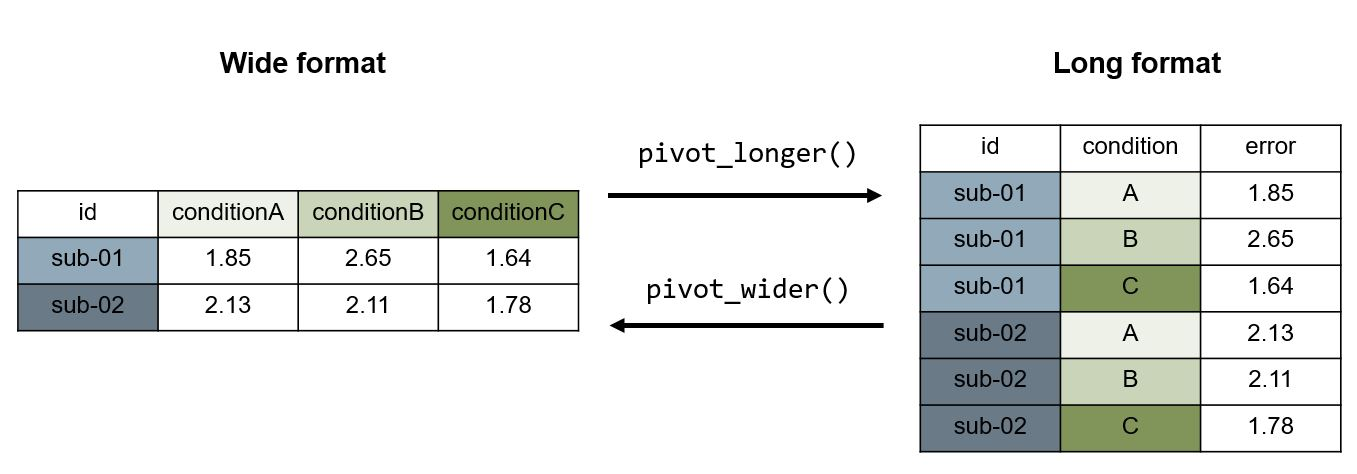
\includegraphics{imgs/widelongformat.JPG}

}

\end{figure}

\begin{center}\rule{0.5\linewidth}{0.5pt}\end{center}

\begin{tcolorbox}[enhanced jigsaw, rightrule=.15mm, colframe=quarto-callout-tip-color-frame, breakable, opacityback=0, bottomrule=.15mm, arc=.35mm, left=2mm, leftrule=.75mm, toprule=.15mm, colback=white]
\begin{minipage}[t]{5.5mm}
\textcolor{quarto-callout-tip-color}{\faLightbulb}
\end{minipage}%
\begin{minipage}[t]{\textwidth - 5.5mm}

\textbf{Questions}\vspace{2mm}

In our example data set we have 4 columns (\texttt{id},
\texttt{condition}, \texttt{x}, \texttt{y}) and 1846 rows. What format
is this?

What data format does your own data set have?

\end{minipage}%
\end{tcolorbox}

\begin{Shaded}
\begin{Highlighting}[]
\FunctionTok{glimpse}\NormalTok{(d)}
\end{Highlighting}
\end{Shaded}

\begin{verbatim}
Rows: 568
Columns: 4
$ id        <int> 1, 2, 3, 4, 5, 6, 7, 8, 9, 10, 11, 12, 13, 14, 15, 16, 17, 1~
$ condition <chr> "away", "away", "away", "away", "away", "away", "away", "awa~
$ x         <dbl> 32.33111, 53.42146, 63.92020, 70.28951, 34.11883, 67.67072, ~
$ y         <dbl> 61.411101, 26.186880, 30.832194, 82.533649, 45.734551, 37.11~
\end{verbatim}

\hypertarget{pivot_wider}{%
\subsection{\texorpdfstring{\texttt{pivot\_wider()}}{pivot\_wider()}}\label{pivot_wider}}

With
\texttt{pivot\_wider(data,\ id\_cols\ =\ ,\ names\_from\ =\ ,\ values\_from\ =\ ,\ ...)}
you can transform your data from \emph{long} to \emph{wide} format.

\textbf{\emph{Example}}

\begin{Shaded}
\begin{Highlighting}[]
\NormalTok{d\_wide }\OtherTok{\textless{}{-}}\NormalTok{ d }\SpecialCharTok{|\textgreater{}} \FunctionTok{pivot\_wider}\NormalTok{(}\AttributeTok{id\_cols =}\NormalTok{ id, }\AttributeTok{names\_from =}\NormalTok{ condition, }\AttributeTok{names\_glue =} \StringTok{"\{condition\}\_\{.value\}"}\NormalTok{, }\AttributeTok{values\_from =} \FunctionTok{c}\NormalTok{(x, y))}
\FunctionTok{glimpse}\NormalTok{(d\_wide)}
\end{Highlighting}
\end{Shaded}

\begin{verbatim}
Rows: 142
Columns: 9
$ id         <int> 1, 2, 3, 4, 5, 6, 7, 8, 9, 10, 11, 12, 13, 14, 15, 16, 17, ~
$ away_x     <dbl> 32.33111, 53.42146, 63.92020, 70.28951, 34.11883, 67.67072,~
$ bullseye_x <dbl> 51.20389, 58.97447, 51.87207, 48.17993, 41.68320, 37.89042,~
$ circle_x   <dbl> 55.99303, 50.03225, 51.28846, 51.17054, 44.37791, 45.01027,~
$ dino_x     <dbl> 55.3846, 51.5385, 46.1538, 42.8205, 40.7692, 38.7179, 35.64~
$ away_y     <dbl> 61.411101, 26.186880, 30.832194, 82.533649, 45.734551, 37.1~
$ bullseye_y <dbl> 83.33978, 85.49982, 85.82974, 85.04512, 84.01794, 82.56749,~
$ circle_y   <dbl> 79.27726, 79.01307, 82.43594, 79.16529, 78.16463, 77.88086,~
$ dino_y     <dbl> 97.1795, 96.0256, 94.4872, 91.4103, 88.3333, 84.8718, 79.87~
\end{verbatim}

\hypertarget{pivot_longer}{%
\subsection{\texorpdfstring{\texttt{pivot\_longer()}}{pivot\_longer()}}\label{pivot_longer}}

With \texttt{pivot\_longer(data,\ cols\ =\ ,\ names\_to\ =\ ,\ ...)} you
can transform your data from \emph{wide} to \emph{long} format.

With \texttt{cols} you specify the columns of the wide dataframe you
want to bring into long format. With \texttt{names\_to} you specify how
the new variables (colums) are named (enter them with \texttt{"}). With
\texttt{names\_sep}you can specify, if two variables should be extracted
from the existing column.

\textbf{\emph{Example}}

\begin{Shaded}
\begin{Highlighting}[]
\NormalTok{d\_long }\OtherTok{\textless{}{-}}\NormalTok{ d\_wide }\SpecialCharTok{|\textgreater{}} \FunctionTok{pivot\_longer}\NormalTok{(}\AttributeTok{cols =}\NormalTok{ away\_x}\SpecialCharTok{:}\NormalTok{dino\_y, }\AttributeTok{names\_to =} \FunctionTok{c}\NormalTok{(}\StringTok{"condition"}\NormalTok{, }\StringTok{"measure"}\NormalTok{), }\AttributeTok{names\_sep =} \StringTok{"\_"}\NormalTok{)}
\FunctionTok{glimpse}\NormalTok{(d\_long)}
\end{Highlighting}
\end{Shaded}

\begin{verbatim}
Rows: 1,136
Columns: 4
$ id        <int> 1, 1, 1, 1, 1, 1, 1, 1, 2, 2, 2, 2, 2, 2, 2, 2, 3, 3, 3, 3, ~
$ condition <chr> "away", "bullseye", "circle", "dino", "away", "bullseye", "c~
$ measure   <chr> "x", "x", "x", "x", "y", "y", "y", "y", "x", "x", "x", "x", ~
$ value     <dbl> 32.33111, 51.20389, 55.99303, 55.38460, 61.41110, 83.33978, ~
\end{verbatim}

\begin{tcolorbox}[enhanced jigsaw, rightrule=.15mm, colframe=quarto-callout-tip-color-frame, breakable, opacityback=0, bottomrule=.15mm, arc=.35mm, left=2mm, leftrule=.75mm, toprule=.15mm, colback=white]
\begin{minipage}[t]{5.5mm}
\textcolor{quarto-callout-tip-color}{\faLightbulb}
\end{minipage}%
\begin{minipage}[t]{\textwidth - 5.5mm}

\textbf{Rule of thumb}\vspace{2mm}

\begin{itemize}
\item
  Variables/factors should have a column (e.g.~the variables you want to
  enter in your model formula).
\item
  Factor levels (e.g.~condition levels such as \texttt{away}) should be
  coded within rows.
\end{itemize}

\end{minipage}%
\end{tcolorbox}

\hfill\break

\hypertarget{choose-variables-in-data-sets}{%
\section{Choose variables in data
sets}\label{choose-variables-in-data-sets}}

If you want to use only some variables or observations you can use
\texttt{select()} and \texttt{filter()}:

\hypertarget{select}{%
\subsection{\texorpdfstring{\texttt{select()}}{select()}}\label{select}}

With \texttt{select(.data,\ variablename,\ ...)} you can choose
variables you want to keep. This is helpful if you have large data files
and not all variables are used for the analysis. You can also delete
variables from the dataset (e.g.~for anonymization) with \texttt{!} in
front of the variable name.

\textbf{\emph{Example}}

If we for example only need variables \texttt{condition} and \texttt{x}
we can create a new more simple data set:

\begin{Shaded}
\begin{Highlighting}[]
\CommentTok{\# only keep variables condition and x without using a pipe}
\NormalTok{d\_simpler }\OtherTok{\textless{}{-}} \FunctionTok{select}\NormalTok{(d, condition, x)}

\CommentTok{\# only keep variables condition and x using a pipe}
\NormalTok{d\_simpler }\OtherTok{\textless{}{-}}\NormalTok{ d }\SpecialCharTok{|\textgreater{}} \FunctionTok{select}\NormalTok{(condition, x)}

\CommentTok{\# keep all variable except x}
\NormalTok{d\_simpler }\OtherTok{\textless{}{-}}\NormalTok{ d }\SpecialCharTok{|\textgreater{}} \FunctionTok{select}\NormalTok{(}\SpecialCharTok{!}\NormalTok{x)}
\end{Highlighting}
\end{Shaded}

\hypertarget{filter}{%
\subsection{\texorpdfstring{\texttt{filter()}}{filter()}}\label{filter}}

With \texttt{filter(.data,\ filter,\ ...)} you can choose observations
you want to keep or delete from the data set. For this you have to
specify your filter.

\textbf{\emph{Example}}

\begin{Shaded}
\begin{Highlighting}[]
\CommentTok{\# only keep observations where dataset is "star"}
\NormalTok{d\_filtered }\OtherTok{\textless{}{-}} \FunctionTok{filter}\NormalTok{(d, condition }\SpecialCharTok{==} \StringTok{"star"}\NormalTok{)}

\CommentTok{\# or with the pipe}
\NormalTok{d\_filtered }\OtherTok{\textless{}{-}}\NormalTok{ d }\SpecialCharTok{|\textgreater{}} \FunctionTok{filter}\NormalTok{(condition }\SpecialCharTok{==} \StringTok{"star"}\NormalTok{)}

\CommentTok{\# only keep observations where dataset is NOT "star"}
\NormalTok{d\_filtered }\OtherTok{\textless{}{-}}\NormalTok{ d }\SpecialCharTok{|\textgreater{}} \FunctionTok{filter}\NormalTok{(condition }\SpecialCharTok{!=} \StringTok{"star"}\NormalTok{)}

\CommentTok{\# only keep observations where x is more than 50 (e.g. for filtering response times)}
\NormalTok{d\_filtered }\OtherTok{\textless{}{-}}\NormalTok{ d }\SpecialCharTok{|\textgreater{}} \FunctionTok{filter}\NormalTok{(x }\SpecialCharTok{\textgreater{}} \DecValTok{50}\NormalTok{)}

\CommentTok{\# only keep observations where x is more than 50 (e.g. for filtering response times)}
\NormalTok{d\_filtered }\OtherTok{\textless{}{-}}\NormalTok{ d }\SpecialCharTok{|\textgreater{}} \FunctionTok{filter}\NormalTok{(x }\SpecialCharTok{\textgreater{}} \DecValTok{50} \SpecialCharTok{\&}\NormalTok{ x }\SpecialCharTok{\textless{}} \DecValTok{60}\NormalTok{)}

\CommentTok{\# use several filters}
\NormalTok{d\_filtered }\OtherTok{\textless{}{-}}\NormalTok{ d }\SpecialCharTok{|\textgreater{}} 
    \FunctionTok{filter}\NormalTok{(condition }\SpecialCharTok{==} \StringTok{"star"}\NormalTok{) }\SpecialCharTok{|\textgreater{}}
    \FunctionTok{filter}\NormalTok{(x }\SpecialCharTok{\textless{}} \DecValTok{50}\NormalTok{)}
\end{Highlighting}
\end{Shaded}

\hypertarget{create-and-manipulate-variables}{%
\section{Create and manipulate
variables}\label{create-and-manipulate-variables}}

Here we look at functions with which we can generate new variables
and/or alter existing ones.

\hypertarget{mutate}{%
\subsection{\texorpdfstring{\texttt{mutate()}}{mutate()}}\label{mutate}}

The \texttt{mutate(.data,\ …)} function is used to generate or alter
variables in a data frame using the pipe.

\textbf{\emph{Example}}

\begin{Shaded}
\begin{Highlighting}[]
\CommentTok{\# generate new variables}
\NormalTok{d\_altered }\OtherTok{\textless{}{-}}\NormalTok{ d }\SpecialCharTok{|\textgreater{}}
    \FunctionTok{mutate}\NormalTok{(}\AttributeTok{num\_variable =} \FloatTok{1.434}\NormalTok{,}
           \AttributeTok{chr\_variable =} \StringTok{"1.434"}\NormalTok{,}
           \AttributeTok{sumofxy\_variable =}\NormalTok{ x }\SpecialCharTok{+}\NormalTok{ y,}
           \AttributeTok{copy\_variable =}\NormalTok{ condition)}

\CommentTok{\# alter exisiting variables}
\NormalTok{d\_altered }\OtherTok{\textless{}{-}}\NormalTok{ d\_altered }\SpecialCharTok{|\textgreater{}}
    \FunctionTok{mutate}\NormalTok{(}\AttributeTok{num\_variable =}\NormalTok{ num\_variable }\SpecialCharTok{*} \DecValTok{1000}\NormalTok{) }\CommentTok{\# e.g. to change seconds to milliseconds}
\end{Highlighting}
\end{Shaded}

\hypertarget{case_when}{%
\subsection{\texorpdfstring{\texttt{case\_when()}}{case\_when()}}\label{case_when}}

If we want to generate variables conditioned on existing data we can use
\texttt{case\_when()}.

\begin{Shaded}
\begin{Highlighting}[]
\NormalTok{d\_condvariables }\OtherTok{\textless{}{-}}\NormalTok{ d }\SpecialCharTok{|\textgreater{}}
    \FunctionTok{mutate}\NormalTok{(}\AttributeTok{cond\_variable =} \FunctionTok{case\_when}\NormalTok{(x }\SpecialCharTok{\textgreater{}} \DecValTok{50} \SpecialCharTok{\textasciitilde{}} \StringTok{"higher"}\NormalTok{,}
\NormalTok{                                     x }\SpecialCharTok{\textless{}=} \DecValTok{50} \SpecialCharTok{\textasciitilde{}} \StringTok{"lower"}\NormalTok{,}
                                     \AttributeTok{.default =} \ConstantTok{NA}\NormalTok{))}
\end{Highlighting}
\end{Shaded}

\hypertarget{as.factor-as.numeric}{%
\subsection{\texorpdfstring{\texttt{as.factor()}, \texttt{as.numeric()},
\ldots{}}{as.factor(), as.numeric(), \ldots{}}}\label{as.factor-as.numeric}}

For changing the variable class we can use these functions. It makes
sense to adjust variable classes at the beginning of the data pipeline,
as it will make a difference for plots as well as models if a variable
is entered categorical or numerical. Subject IDs for example are often
numerical values but are actually categorical.

\begin{Shaded}
\begin{Highlighting}[]
\CommentTok{\# change to factor (categorical/nominal)}
\NormalTok{d }\OtherTok{\textless{}{-}}\NormalTok{ d }\SpecialCharTok{|\textgreater{}} 
    \FunctionTok{mutate}\NormalTok{(}\AttributeTok{id =} \FunctionTok{as.factor}\NormalTok{(id))}
\end{Highlighting}
\end{Shaded}

\hypertarget{group-and-summarise-data}{%
\section{Group and summarise data}\label{group-and-summarise-data}}

\hypertarget{group_by-and-summarise}{%
\subsection{\texorpdfstring{\texttt{group\_by()} and
\texttt{summarise()}}{group\_by() and summarise()}}\label{group_by-and-summarise}}

With these functions you can group a data frame by factor levels and
calculate mean scores or else.

\begin{Shaded}
\begin{Highlighting}[]
\CommentTok{\# look at each individual}
\NormalTok{d }\SpecialCharTok{|\textgreater{}} \FunctionTok{group\_by}\NormalTok{(id) }\SpecialCharTok{|\textgreater{}}
    \FunctionTok{summarise}\NormalTok{(}\AttributeTok{mean\_x =} \FunctionTok{mean}\NormalTok{(x),}
              \AttributeTok{mean\_y =} \FunctionTok{mean}\NormalTok{(y))}
\end{Highlighting}
\end{Shaded}

\begin{verbatim}
# A tibble: 142 x 3
   id    mean_x mean_y
   <fct>  <dbl>  <dbl>
 1 1       48.7   80.3
 2 2       53.5   71.7
 3 3       53.3   73.4
 4 4       53.1   84.5
 5 5       40.2   74.1
 6 6       47.3   70.6
 7 7       44.3   84.2
 8 8       44.6   65.6
 9 9       43.2   78.0
10 10      38.9   61.7
# i 132 more rows
\end{verbatim}

\begin{Shaded}
\begin{Highlighting}[]
\CommentTok{\# look at each individual in each condition}
\NormalTok{d\_sum }\OtherTok{\textless{}{-}}\NormalTok{ d }\SpecialCharTok{|\textgreater{}} \FunctionTok{group\_by}\NormalTok{(id, condition) }\SpecialCharTok{|\textgreater{}}
    \FunctionTok{summarise}\NormalTok{(}\AttributeTok{mean\_x =} \FunctionTok{mean}\NormalTok{(x),}
              \AttributeTok{sd\_x =} \FunctionTok{sd}\NormalTok{(x),}
              \AttributeTok{mean\_y =} \FunctionTok{mean}\NormalTok{(y),}
              \AttributeTok{sd\_y =} \FunctionTok{sd}\NormalTok{(x))}
\end{Highlighting}
\end{Shaded}

\begin{verbatim}
`summarise()` has grouped output by 'id'. You can override using the `.groups`
argument.
\end{verbatim}

\begin{Shaded}
\begin{Highlighting}[]
\FunctionTok{glimpse}\NormalTok{(d\_sum)}
\end{Highlighting}
\end{Shaded}

\begin{verbatim}
Rows: 568
Columns: 6
Groups: id [142]
$ id        <fct> 1, 1, 1, 1, 2, 2, 2, 2, 3, 3, 3, 3, 4, 4, 4, 4, 5, 5, 5, 5, ~
$ condition <chr> "away", "bullseye", "circle", "dino", "away", "bullseye", "c~
$ mean_x    <dbl> 32.33111, 51.20389, 55.99303, 55.38460, 53.42146, 58.97447, ~
$ sd_x      <dbl> NA, NA, NA, NA, NA, NA, NA, NA, NA, NA, NA, NA, NA, NA, NA, ~
$ mean_y    <dbl> 61.41110, 83.33978, 79.27726, 97.17950, 26.18688, 85.49982, ~
$ sd_y      <dbl> NA, NA, NA, NA, NA, NA, NA, NA, NA, NA, NA, NA, NA, NA, NA, ~
\end{verbatim}

\bookmarksetup{startatroot}

\hypertarget{data-visualization}{%
\chapter{Data visualization}\label{data-visualization}}

\begin{itemize}
\item
  Data visualisation mit \texttt{ggplot} - Package (Gerda)

  \begin{itemize}
  \item
    different Graphs
  \item
    mapping: \texttt{aes()}
  \item
    Geoms: \texttt{geom\_boxplot()}, \texttt{geom\_violin()}, \ldots{}
  \item
    Colors, Shapes, Labels, \ldots{}
  \end{itemize}
\end{itemize}

Further ressources:

https://rstudio-connect.psy.gla.ac.uk/plotdemo/



\end{document}
